\chapter{BACKGROUND}
\label{background}

<<<<<<< Updated upstream
=======
<<<<<<< HEAD
This thesis combines several topics and applies multiple computer sciences and cheminformatics studies. This chapter provides insight into this study's techniques and terminology: homogeneous and heterogeneous graphs, graph representation learning, language model-based representation learning, and evaluation metrics. 

\section{Graphs}
A graph $G = (V, \varepsilon)$ is defined by a set of nodes $V$ and a set of edges $\varepsilon$ between these nodes as going from node $u \in V$ to node $v \in V$ as $(u,v) \in \varepsilon$ \cite{biggs1993algebraic}. In this thesis, we concern only simple graphs, i.e., there exists at most one edge between each pair of nodes and no edges between a node and itself. Moreover, all edges are undirected, so $(u,v) \in \varepsilon \longleftrightarrow (v,u) \in \varepsilon$. A graph has a single type of edge or different types of edges. In a multi-relational graph the edge notation can be extended as $(u,\tau,v) \in \varepsilon$ to include the relation type $\tau$ \cite{hamilton2020graph}. Throughout the thesis, we consider two important subsets of graphs; graphs with single and multiple relation types, \textit{i.e.}, homogeneous and heterogeneous, respectively. 

\begin{figure}[h]
    \centering
        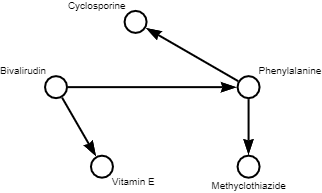
\includegraphics[width=0.5\linewidth]{chapters/background/figures/ddi.png} 
    \caption{Homogeneous drug-drug interaction graph.}
    \label{fig:sample_ddi}
\end{figure}
A graph is homogeneous when all the nodes represent the same type of instances, and all the edges represent the same type of relations \cite{gardiner1976homogeneoys, gardiner1978homogeneity}. For instance, a drug-drug interaction network is a homogeneous graph consisting of drugs and the connections between these drugs, representing the same type of entity. 

Figure \ref{fig:sample_ddi} shows a homogeneous drug-drug interaction graph with five drugs; Bivaluridin, Cyclosporine, Methyclothoazide, Vitamin E, and Phenylalanine; and the edges represent the interaction between drug pairs. For example, Cyclosporine interacts with Phenylalanine, and this interaction is extracted from the DrugBank database, depicting the increased risk of bleeding when Cyclosporine is consumed with Phenylalanine \cite{ihlefeldt2014polymorphs}. 


\begin{figure}[h]
    \centering
        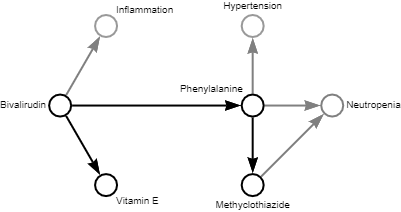
\includegraphics[width=0.65\linewidth]{chapters/background/figures/dda.png} 
    \caption{Heterogeneous drug-disease association graph.}
    \label{fig:sample_dda}
\end{figure}
A graph is heterogeneous if the set of nodes can be partitioned into disjoint sets $V = V_{1} \cup V_{2} \cup ... \cup V_{k} $ where $V_{i} \cap V_{j} = \emptyset , \forall i \neq j$ \cite{sun2013mining}. For instance, the drug-disease network is a heterogeneous graph consisting of two types of nodes as drugs and diseases, and two types of edges represent the treatment relationship between drug nodes and disease nodes, and similarly, the polypharmacy side effect that occurs only between two drug nodes. 

Figure \ref{fig:sample_dda} shows a heterogeneous drug-disease association graph with four drugs; Bivaluridin, Phenylalanine, Vitamin E, and Methyclothoazide, three diseases; inflammation, hypertension, and Neutropenia, and two types of edges; drug interacts with a drug and drug associates with a disease. For instance, Methyclothiazide interacts with Phenylalanine, and both drugs associate with Neutropenia. This relation depicts that the risk or severity of Neutropenia can be increased when Methyclothiazide is combined with Phenylalanine \cite{ruiz2022primary}. 




\section{Graph Representation Learning}
\label{section:graph_rep_le}
The rapid development of molecular biology, bioinformatics, and cheminformatics and the increase in the available data has led to the modeling of the biological components as nodes and the interactions between nodes as edges of graphs \cite{mason2007graph, pavlopoulos2011using, ricard2006biological}. In the case of drug discovery and disease treatment, it is crucial to examine the interactions between drug-drug, drug-disease, drug-protein, and protein-disease \cite{daminelli2012drug, davis2009comparative}. These interactions can be formed as heterogeneous graphs and used in knowledge extraction. Traditional machine learning algorithms use the data represented in the Euclidean domain, such as 1D sequences of proteins, 2D biomedical images, or 3D protein structures. However, graphs form a non-Euclidean domain and create a challenge due to their complex topological structure \cite{bronstein2017geometric, asif2021graph}, diverse node connections, and arbitrary neighbor size. To address these challenges, graph representation learning is employed. Graph representation learning or graph embedding learns the low-dimensional representations of nodes or edges used in downstream graph analytical tasks or machine learning tasks such as node classification, link prediction, and graph classification.

The graph-based distributed representation learning method represents the chemicals and proteins. In general, this set of methods represents data that cannot be expressed in Euclidean space as a graph, and it aims to learn distributed vectors that reflect the semantic connections in the graph for nodes and edges \cite{wu2019comprehensive}. %Using the compiled data (See details in Chapter \ref{chapter:dataset_preparation}), we model protein, ligand, disease, and side effect information and the extracted language-based information as different node types in a graph. 

One of the essential advantages of this approach is that it can express the relationships between different types of nodes. The relationship between each node corresponds to different relationships. Graph-based representation vectors are learned for proteins and chemicals using the heterogeneous graph structure. In this heterogeneous graph, when distributed representations for chemicals and proteins are learned, the relationships of nodes with different concepts such as disease and side effects are also included in the representations. In this way, the received vectors become richer in terms of information. 

To learn the distributed representation vectors, Metapath2Vec \cite{dong2017metapath2vec, pal2016deep} is employed, which is a framework to learn representations of heterogeneous graphs. It is a neural network model that is designed to capture the rich semantics embedded in heterogeneous graphs by exploiting different types of relationships and meta-paths among nodes. To generate meaningful representations, it considers different semantics of relations, i.e., different meta-paths, the sequence of node/edge types that denote relationships between node pairs.

The word2vec model is proposed to learn the distributed representations of words within a corpus \cite{mikolov2013efficient, mikolov2013distributed}. After that, DeepWalk \cite{perozzi2014deepwalk}, and node2vec \cite{grover2016node2vec} models were proposed, aiming to map the word-context concept of the word2vec model into a network. DeepWalk and node2vec models use random walks to map the word-context concept and utilize the skip-gram model to learn the node representation in a homogeneous network. Their objective is to maximize the network probability \cite{mikolov2013distributed, perozzi2014deepwalk, grover2016node2vec} as
\begin{equation}
    arg \max_{\theta} \prod_{v \in V}^{} \prod_{c \in N(V)}^{} p(c|v;\theta),
    \label{eq:argmax}
\end{equation}
\noindent where $N(v)$ denotes the node $v$'s neighborhood, in which $v$'s one-hop neighbors, and $p(c|v;\theta)$ defines the conditional probability of a context node $c$ given node $v$.

Metapath2Vec formalizes the representation learning problem in heterogeneous networks by leveraging the definitions in \cite{dong2017metapath2vec, sun2013pathselclus} as follows:

A heterogeneous network is a graph $G = (V, E, T)$ in which node $v$ is associated with edge $e$ with mapping functions $\phi(v) : V \to T_{V}$ and $\varphi(e) : E \to T_{E}$, respectively. Heterogeneous network representation learning aims to learn the d-dimensional representation $X \in R^{|V|\times d}, d \ll |V|$, given a heterogeneous network $G$, that is able to capture the topological and semantic relations among them. Therefore, the resulting representation is a low-dimensional matrix $X$, with the $v^{th}$  row corresponding to the representation of node $v$. Regardless of the node types in $V$, representations of each node are mapped into the same latent space. 

Similar to word2vec, Metapath2Vec introduces the heterogeneous skip-gram model for heterogeneous networks to model the heterogeneous neighborhood of a node. Therefore, Metapath2Vec aims to maximize the probability of having the heterogeneous context $N_{t}(v), t \in T_{V}$ given a node $v$ as
\begin{equation}
    arg \max_{\theta} \sum_{v \in V}^{} \sum_{t \in T_{V} }^{} \sum_{c_{t} \in N_{t}(V)}^{} p(c_{t}|v;\theta),
\label{eq:context}
\end{equation}
\noindent where $N_{t}(v)$ denotes the node $v$'s neighborhood with the $t^{th}$ type of nodes. The $p(c_{t}|v;\theta)$ is a softmax function \cite{bengio2013representation, mikolov2013distributed} formulated as
\begin{equation}
    p(c_{t}|v;\theta) = \frac{e^{X_{c_{t}}}.X_{v}}{\sum_{u \in V}^{} e^{X_{u}}.X_{v}},
\label{eq:softmax}
\end{equation}
\noindent where $X_{v}$ is the $v^{th}$ row of $X$, corresponding to the embedding vector for node $v$. The word2vec also introduces negative sampling \cite{mikolov2013distributed} for optimization. A small set of words are sampled from the corpus with negative sampling to compute the softmax. Same technique is also applied for Metapath2Vec, and Equation (\ref{eq:context}) is updated as
\begin{equation}
    log\sigma(X_{c_{t}}.X_{v}) + \sum_{m=1}^{M} \mathbb{E}_{u^{m}\sim P(u)}[log\sigma(-X_{u^{m}}.X_{v})],
\label{eq:update_softmax}
\end{equation}
\noindent where $M$ is the negative sample size, $\sigma (x) = \frac{1}{1+e^{-x}}$ and $P(u)$ is the pre-defined distribution in which node $u^{m}$ is drew from $M$ times.

In order to transform heterogeneous network structures into metapath2vec's skip-gram, the model designs a meta-path-based random walks, and generate paths. A meta-path schema is a path, denoted as $V_{1} \xrightarrow[]{R_{1}} V_{2} \xrightarrow[]{R_{2}}\cdots V_{t} \xrightarrow[]{R_{t}} V_{t+1} \cdots \xrightarrow[]{R_{l-1}} V_{l}$, where $R = R_{1} \circ R_{2} \circ \cdots \circ R_{l-1}$ defines the composite relations between node types $V_{1}$ and $V_{l}$ \cite{sun2012mining}.

As shown above, Metapath2Vec uses random walks guided by meta-paths to generate heterogeneous node sequences rich in semantics and structural information, and then it designs a heterogeneous skip-gram model to preserve the node $v$'s proximity to its neighborhood nodes. It uses Equation \ref{eq:update_softmax} to calculate the similarity between a node and its neighbors.

Based on Metapath2Vec, several variants have been proposed. For instance, BHIN2vec \cite{lee2019bhin2vec} proposes an extension to the skip-gram technique in order to balance the influence of different relation types on node embeddings. HHNE \cite{wang2019hyperbolic} performs random walks in hyperbolic spaces. Another method, Hin2Vec \cite{fu2017hin2vec}, combines first-order and high-order relations to capture the heterogeneity of graphs and carries out multiple relation prediction tasks to learn the node embeddings jointly. This thesis employs Metapath2Vec since its code is freely available to use and easy to adapt to homogeneous and heterogeneous graphs.

\section{Language Model-Based Representation Learning}
\label{section:languagE_rep_le}
Conventional Natural Language Processing (NLP) requires feature engineering, thus considerable expertise. Likewise, representation learning aims to automatically learn representations of row data to be fed as input to classification or prediction tasks as useful information. A typical example of representation learning approaches is deep learning \cite{goodfellow2016deep} since the output of each intermediary layer can be considered as a representation of the input data. Deep learning algorithms represent each object with a low-dimensional, real-valued dense vector called distributed representation or embedding. When two objects are projected into a unified low-dimensional semantic space, the geometric distance between these objects in the semantic space indicates their semantic relatedness. Therefore, the semantic meaning of an object is related to its close neighbors \cite{liu2020representation}. 

One of the exciting approaches to distributed representation in NLP is Neural Probabilistic Language Model (NPLM) \cite{bengio2001neural}. A language model is created to predict the joint probability of word sequences. In NPLM, a distributed vector is assigned for each word at first, then using a neural network, the next word is predicted. In the end, it learns how to model the joint probability of sentences and outputs the word embeddings as learned parameters. Some of the famous methods inspired by NPLM are word2vec \cite{mikolov2013distributed}, GloVe \cite{bojanowski2017enriching}, and fastText \cite{pennington2014glove}, all of which are very efficient to train. 

With the growing number of data in the corpus and the parameters, ELMo \cite{devlin2018bert}, and BERT \cite{peters2018deep} models have become more popular. Rather than assigning a fixed distributed vector to each word as in word2vec, ELMo and BERT use multilayer neural networks to calculate dynamic representations of words. Most importantly, they consider a word's context while learning the representation. 

BERT-like models are also called Pre-trained Language Models (PLM) because they are pre-trained through text modeling objectives on large corpora and fine-tuned the model on downstream tasks. 
%Due to experiments that show PLMs encode linguistic knowledge and patterns into their multilayer network parameters, we employed these models in this thesis \cite{liu2019linguistic, hewitt2019structural}. Similar to the natural languages, SMILES and amino acid sequences are typical unstructured information, and to initialize our graph-based representation learning models we leveraged transformer variants pre-trained on large datasets such as ProtBERT \cite{Elnaggar2020.07.12.199554}, ChemBERTa \cite{chithrananda2020chemberta}, and BioBERT \cite{lee2020biobert}. 
BERT is a bi-directional transformer that can learn a language representation from a large amount of unlabeled textual data and then fine-tune it for certain machine learning applications. ProtBERT \cite{prot_bert, Elnaggar2020.07.12.199554} is a protein sequence-pre-trained model with a masked language modeling objective. It is based on the BERT model, which is self-supervised and pre-trained on a vast corpus of protein sequences. This implies it was pre-trained on raw protein sequences only, with no human labeling, and used an automatic mechanism to generate inputs and labels from those sequences. To initialize the distributional representations of proteins, we leverage the ProtBERT model. 

We adopted the ChemBERTa \cite{chithrananda2020chemberta} model, which was pre-trained on 10M PubChem substances using BPE tokenization \cite{sennrich2015neural}, to initialize the distributional representations of chemicals. ChemBERTa is based on the transformer and pre-trained with masked language modeling, similar to ProtBERT.

To initialize the distributional representations of diseases and side effects, we employed the BioBERT \cite{lee2020biobert} model. It is a domain-specific language representation model pre-trained on large-scale biomedical corpora, the same as the preceding models.

%\section{Affinity Prediction}
%Deep learning approaches showed performance improvement compared to machine learning approaches because they use network-based methods that are not reliant on the availability of the 3D protein structure \cite{lounkine2012large}. Some deep learning approaches for measuring drug-target affinity prediction include DeepDTA \cite{ozturk2018deepdta}, PADME \cite{feng2018padme}, WideDTA \cite{ozturk2019widedta}, and DeepAffinity \cite{karimi2019deepaffinity}. DeepDTA receives drug data in the form of SMILES, in which the amino acid sequence for protein input data is entered. WideDTA is a deep learning method based on multi-layered convolutional neural networks for determining binding affinity that uses ligand SMILES, amino acid sequences, ligand maximum common substructure (LMCS), and protein domains and motifs as input data \cite{gao2018interpretable}.

The DeepDTA model revealed the difficulties of modeling proteins using their sequences, which was one of the study's most intriguing findings \cite{ozturk2018deepdta}. In the affinity prediction task, the CNN module was not as good at describing proteins when modeled separately by CNN-based modules as it was with SMILES. 

The WideDTA model utilizes the protein sequence and ligand SMILES string to address this issue by representing them as a set of words. Moreover, to better represent the interaction, the WideDTA model incorporated many kinds of text-based information. Although the addition of text-based information such as protein domain and motif information, the protein representation and thus prediction performance were unable to create a statistically significant gain in predictive power. Inspired by this, we expand the DeepDTA model by integrating more information and creating better and semantically meaningful representations for chemicals and proteins.

\section{Evaluation Metrics}
\label{section:evaluation}
To evaluate the performance of the graph-based and language-based models, we utilize four metrics: Concordance Index (CI) \cite{gonen2005concordance}, R-squared ($R^2$), Mean Square Error (MSE), Root Mean Square Error (RMSE), and Cosine Similarity. These five metrics will be introduced in the following.

\subsection{Concordance Index}
In the DTA prediction task, the Concordance Index (CI) can be utilized as an evaluation metric for prediction correctness, as described in KronRLS \cite{pahikkala2015toward}. For continuous values, CI is a ranking metric. The CI is used to determine whether two random drug-target combinations' projected binding affinity values were predicted in the same order as their actual values or not. CI is calculated as
\begin{equation}
    CI =  \frac{1}{Z}\sum_{s_{i} > s_{j}}^{}h(b_{i}-b_{j}),
\end{equation}
\noindent where $b_i$ is the prediction value for the larger affinity $s_i$, $b_j$ is the prediction value for the smaller affinity $s_j$, $Z$ is a normalization constant equal to the number of data pairs with different label values. The CI spans from 0 to 1.0, with 1.0 indicating perfect prediction accuracy and 0.5 indicating a random predictor. The Heaviside function, $h(x)$, is \cite{gonen2005concordance} step function, which is discontinued and it is defined as
=======
>>>>>>> Stashed changes
\section{Graphs}
A graph $G = (V, \varepsilon)$ is defined by a set of nodes $V$ and a set of edges $E$ between these nodes as going from node $u \in V$ to node $v \in V$ as $(u,v) \in \varepsilon$. In this thesis, we concern only simple graphs, i.e., there exists at most one edge between each pair of nodes, and no edges between  a node and itself. Moreover, all edges are undirected, so $(u,v) \in \varepsilon \longleftrightarrow (u,v) \in \varepsilon$. A graph has a single type of edge or different type of edges. In a multi-relational graph the edge notation can be extended as $(u,\tau,v) \in \varepsilon$ to include the relation type $\tau$ \cite{hamilton2020graph}. Throughout the thesis we consider two important subsets of graphs; homogeneous and heterogeneous i.e., graphs with single and multiple relation types respectively. 

Graph is homogeneous when all the nodes represents the instances of the same type and all the edges represents the same type of relations. For instance, drug-drug interaction network is a homogeneous graph consisting of drugs and the connections between drugs, representing the same type of entity. Figure \ref{fig:sample_ddi} shows a homogeneous drug-drug interaction graph with five drugs, and the risk or severity of bleeding can be increased when Cyclosporine is combined with Phenylalanine \cite{ihlefeldt2014polymorphs}. 

\begin{figure}
    \centering
        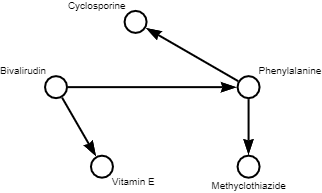
\includegraphics[width=0.5\linewidth]{chapters/background/figures/ddi.png} 
    \caption{Homogeneous Drug-Drug Interaction Graph.}
    \label{fig:sample_ddi}
\end{figure}

Graph is heterogeneous if the set of nodes can be partitioned into disjoint sets $V = V_{1} \cup V_{2} \cup ... \cup V_{k} $ where $V_{i} \cap V_{j} = \emptyset , \forall i \neq j$ \cite{sun2013mining}. For instance, drug-disease network is a heterogeneous graph consisting of two types of nodes as drugs and diseases, and two types of edges representing the \textit{treatment} relation that occurs only between drug nodes and disease nodes, and similarly \textit{polypharmacy side effect} that occurs only between two drug nodes. Figure \ref{fig:sample_ddi} shows a heterogeneous drug-disease association graph with 4 drugs, three disease, and two types of edges. For instance, the risk or severity of neutropenia can be increased when Methyclothiazide is combined with Phenylalanine \cite{ruiz2022primary}. 

\begin{figure}
    \centering
        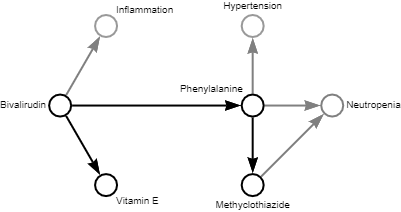
\includegraphics[width=0.65\linewidth]{chapters/background/figures/dda.png} 
    \caption{Heterogeneous Drug-Disease Association Graph.}
    \label{fig:sample_dda}
\end{figure}


\section{Graph Representation Learning}
The rapid development of molecular biology, bioinformatics, and cheminformatics and the increase in the number of available data have led the modeling the biological components as nodes and the interactions between nodes as edges of graphs. In the case of the drug discovery and disease treatment, it is crucial to examine the interactions between drug-drug, drug-disease, drug-protein, and protein-disease \cite{daminelli2012drug, davis2009comparative}. These interactions can be formed as heterogeneous graphs and used in knowledge extraction. Traditional machine learning algorithms use the data represented in Euclidean domain such as 1D sequences of proteins, 2D biomedical image, or 3D protein structure. However, graphs form a non-Euclidean domain and create a challenge due to its complex topological structure, diverse node connections, and arbitrary neighbor size. To address these challenges, graph representation learning is employed. Graph representation learning or graph embedding learns the low-dimensional representations of node or edges that can be used in downstream graph analytics or machine learning tasks such as node classification, and link prediction.

We use graph-based distributional representation learning method to represent the molecules. In general, this set of methods represents data that cannot be expressed in Euclidean space as a graph, and it aims to learn distributed vectors that reflect the semantic connections in the graph for nodes, edges or underlines in this graph \cite{wu2019comprehensive}. One of the most important advantages of this approach is that it can express the relationships between different types of nodes. Using the compiled data (See details in Chapter \ref{chapter:dataset_preparation}) we model protein, ligand, disease and side effect information and the extracted language-based information as different node types in a graph. The relationship between each node corresponds to different relationships such as protein-drug interaction and protein-protein interaction in our graph. By using the heterogeneous graph structure that we have obtained in this way, we learn the graph-based representation vectors for proteins and chemicals. In this heterogeneous graph, when distributional representations for chemicals and proteins are learned, the relationships of nodes with different concepts such as disease and side effects are also included in the representations. In this way, the output of the received vectors becomes richer in terms of information. 

To learn the distributional representation vectors we use MetaPath2Vec \cite{dong2017metapath2vec, pal2016deep}, which is a framework to learn representations of heterogeneous graphs. It is a neural network model that is designed to capture the rich semantics embedded in heterogeneous graphs by exploiting different types of relationships and meta-paths among nodes. To generate meaningful representations, it considers different semantics of relations, i.e., different meta-paths which are the sequence of node/edge types that denote relationships between node pairs.

MetaPath2Vec formalizes the representation learning problem in heterogeneous networks by leveraging the definitions in \cite{dong2017metapath2vec, sun2013pathselclus} as follows:

A heterogeneous network is a graph $G = (V, E, T)$ in which node $v$ is associated with edge $e$ with mapping functions $\phi(v) : V \to T_{V}$ and $\varphi(e) : E \to T_{E}$, respectively. The aim of heterogeneous network representation learning is to learn the d-dimensional representation $X \in R^{|V|\times d}, d \ll |V|$ , given a heterogeneous network $G$, that is able to capture the topological and semantic relations among them. Therefore, the resulting representation is low-dimensional matrix $X$, with the $v^{th}$  row corresponding to the representation of node $v$. Regardless of the node types in $V$, representations of each node are mapped into the same latent space. 

The word2vec model is proposed to learn the distributed representations of words within a corpus \cite{mikolov2013efficient, mikolov2013distributed}. Thereafter, DeepWalk \cite{perozzi2014deepwalk} and node2vec \cite{grover2016node2vec} models proposed, aiming to map the word-context concept of word2vec model into a network. DeepWalk and node2vec models use random walks to map the word-context concept and utilize the skip-gram model to learn the node representation in a homogeneous network. Their objective is to maximize the network probability \cite{mikolov2013distributed, perozzi2014deepwalk, grover2016node2vec}, that is:
\begin{equation}
    arg \max_{\theta} \prod_{v \in V}^{} \prod_{c \in N(V)}^{} p(c|v;\theta)
\end{equation}

where $N(v)$ denotes the node $v$'s neighborhood, in which $v$'s one-hop neighbors, and $p(c|v;\theta)$ defines the conditional probability of a context node $c$ given node $v$.

In the same way, metapath2vec introduces the heterogeneous skip-gram model for heterogeneous networks to model the heterogeneous neighborhood of a node. Therefore, metapath2vec aims to maximize the probability of having the heterogeneous context $N_{t}(v), t \in T_{V}$ given a node $v$:

\begin{equation}
    arg \max_{\theta} \sum_{v \in V}^{} \sum_{t \in T_{V} }^{} \sum_{c_{t} \in N_{t}(V)}^{} p(c_{t}|v;\theta)
\label{eq:context}
\end{equation}

where $N_{t}(v)$ denotes the node $v$'s neighborhood with the $t^{th}$ type of nodes. The $p(c_{t}|v;\theta)$ is a softmax function \cite{bengio2013representation, mikolov2013distributed}, that is:

\begin{equation}
    p(c_{t}|v;\theta) = \frac{e^{X_{c_{t}}}.X_{v}}{\sum_{u \in V}^{} e^{X_{u}}.X_{v}}
\label{eq:softmax}
\end{equation}

where $X_{v}$ is the $v^{th}$ row of $X$, corresponding to the embedding vector for node $v$. Mikolov \textit{et al.} also introduce negative sampling \cite{mikolov2013distributed} for optimization. With negative sampling, a small set of words are sampled from the corpus to construct the softmax. Same technique is also applied for metapath2vec, and Equation \ref{eq:context} is updated as follows:

\begin{equation}
    log\sigma(X_{c_{t}}.X_{v}) + \sum_{m=1}^{M} \mathbb{E}_{u^{m}\sim P(u)}[log\sigma(-X_{u^{m}}.X_{v})]
\end{equation}

where $M$ is the negative sample size, $\sigma (x) = \frac{1}{1+e^{-x}}$ and $P(u)$ is the pre-defined distribution in which node $u^{m}$ is drew from $M$ times.

In order to transform heterogeneous network structures into metapath2vec's skip-gram, that design a meta-path-based random walks, and generate paths. A meta-path schema is a path, denoted as $V_{1} \xrightarrow[]{R_{1}} V_{2} \xrightarrow[]{R_{2}}\cdots V_{t} \xrightarrow[]{R_{t}} V_{t+1} \cdots \xrightarrow[]{R_{l-1}} V_{l}$, where $R = R_{1} \circ R_{2} \circ \cdots \circ R_{l-1}$ defines the composite relations between node types $V_{1}$ and $V_{l}$ \cite{sun2012mining}.

As shown above, metapath2vec uses random walks guided by meta-paths to generate heterogeneous node sequences that are rich in semantics and structural information, then it designs a heterogeneous skip-gram model to preserve the node $v$'s proximity to its neighborhood nodes. It uses Equation \ref{eq:softmax} to calculate the similarity a node and its neighbors.

Based on metapath2vec, several variants have been proposed. For instance, BHIN2vec \cite{lee2019bhin2vec} proposes an extension to the skip-gram technique in order to balance the influence different relation types on node embeddings. HHNE \cite{wang2019hyperbolic} performs random walks in hyperbolic spaces. Another method, Hin2vec \cite{fu2017hin2vec}, combines first-order and high-order relations to capture the heterogeneity of graph and carries out multiple relation prediction tasks to jointly learn the node embeddings. In this thesis we employ metapath2vec since it is simpler and convenient to apply to large heterogeneous graph. Moreover, its code is open, so it is freely available to use and easy to adapt.\footnote{Code available at: https://github.com/apple2373/metapath2vec}

\section{Language Model-Based Representation Vector Learning}
Conventional Natural Language Processing (NLP) requires feature engineering, thus considerable expertise. Likewise, representation learning aims to learn representations of row data automatically to be fed as input to classification or prediction tasks as useful information. A typical example of representation learning approaches is deep learning \cite{goodfellow2016deep}. Deep learning algorithms represent each object with a low-dimensional real-valued dense vectors, named as distributed representation or embedding. When two objects are projected into a unified low-dimensional semantic space, geometric distance between these objects in the semantic space indicates their semantic relatedness. Therefore, the semantic meaning of an object is related to its close neighbors \cite{liu2020representation}.  

One of the exiting approaches of distributed representation in NLP is Neural Probabilistic Language Model (NPLM) \cite{bengio2001neural}. A language model is created to predict the joint probability of word sequences. In NPLM, a distributed vector is assigned for each word at first, then using a neural network, the next word is predicted. In the end, it learns how to model the joint probability of sentences and outputs the word embeddings as learnt parameters. Some of the famous methods inspired by NPLM are word2vec \cite{mikolov2013distributed}, GloVe \cite{bojanowski2017enriching}, and fastText \cite{pennington2014glove}, all of which are very efficient to train. 

With the increasing number of data in corpus and the parameters ELMo \cite{devlin2018bert} and BERT \cite{peters2018deep} models have become more popular. Rather than assigning a fixed distributed vector to each word as in word2vec, ELMo and BERT use multilayer neural networks to calculate dynamic representations of words. Most importantly, they consider a word's context while learning the representation. BERT-like models are also called as Pre-trained Language Models (PLM) because they are pre-trained through modeling objective on large corpora and fine-tuned the model on downstream tasks. 

Due to experiments that show PLMs encode a linguistic knowledge and patterns into their multilayer network parameters we employed these models in this thesis \cite{liu2019linguistic, hewitt2019structural}. Similar to the natural languages, SMILES and amino acid sequences are typical unstructured information, and to initialize our graph-based representation learning models we leveraged transformer variants pre-trained on large datasets such as ProtBERT \cite{Elnaggar2020.07.12.199554}, ChemBERTa \cite{chithrananda2020chemberta}, and BioBERT \cite{lee2020biobert}. 

BERT is a bi-directional transformer that can learn a language representation from a large amount of unlabeled textual data and then fine-tune it for certain machine learning applications. ProtBERT \cite{prot_bert, Elnaggar2020.07.12.199554} is a protein sequence-pre-trained model with a masked language modeling objective. It's based on the BERT model, which is self-supervised and pre-trained on a vast corpus of protein sequences. This implies it was pre-trained on raw protein sequences only, with no human labeling, and used an automatic mechanism to generate inputs and labels from those sequences. To initialize the distributional representations of proteins we leverage the ProtBERT model. 

We adopted the ChemBERTa \cite{chithrananda2020chemberta} model, which was pre-trained on 10M PubChem substances using BPE tokenization \cite{sennrich2015neural}, to initialize the distributional representations of chemicals. ChemBERTa is based on the transformer and has been pre-trained with masked language modeling, similar to ProtBERT.

To initialize the distributional representations of diseases and side effects, we employed the BioBERT \cite{lee2020biobert} model. It's a domain-specific language representation model pre-trained on large-scale biomedical corpora, same like the preceding models.

\section{Affinity Prediction}
Deep learning approaches have outperformed machine learning because they use network-based methods that aren't reliant on the availability of the 3D protein structure \cite{lounkine2012large}. Some deep learning approaches for measuring drug-target affinity prediction include DeepDTA \cite{ozturk2018deepdta}, PADME \cite{feng2018padme}, WideDTA \cite{ozturk2019widedta}, and DeepAffinity \cite{karimi2019deepaffinity}. DeepDTA receives drug data in the form of SMILES, in which the amino acid sequence for protein input data is entered. WideDTA is a deep learning method based on multi-layered convolutional neural networks for determining binding affinity that uses ligand SMILES, amino acid sequences, ligand maximum common substructure (LMCS), and protein domains and motifs as input data \cite{gao2018interpretable}.

The DeepDTA model revealed the difficulties of modeling proteins using their sequences, which was one of the study's most intriguing findings \cite{ozturk2018deepdta}. In the affinity prediction task, the CNN module was not as good at describing proteins when modelled separately by CNN-based modules as it was with SMILES. To address this issue, WideDTA model utilize the protein sequence and ligand SMILES string by representing them as a set of words. Moreover, to provide a better representation of the interaction, the WideDTA model incorporated many kinds of text-based information. Although the addition of text-based information such as protein domain and motif information, the protein representation and thus prediction performance, were unable to create a statistically significant gain in predictive power. Inspired by this, we expand DeepDTA model by integrating more information and create better and semantically meaningful representations for both chemicals and proteins.


\section{Evaluation}

To evaluate the performance of these models, we utilize four metrics: CI \cite{gonen2005concordance}, $R^2$, MSE, and RMSE. These three measures will be introduced in the following.

\subsection{Concordance Index (CI)}
In DTA prediction task, the CI can be utilized as an evaluation metric for prediction accuracy, as described in KronRLS \cite{pahikkala2015toward}. For continuous values, CI is a ranking metric. The CI is used to determine whether two random drug-target combinations' projected binding affinity values were predicted in the same order as their actual values or not. The CI spans from 0.5 to 1.0, with 1.0 indicating perfect prediction accuracy and 0.5 indicating a random predictor. The following formula is used to calculate the CI:
\begin{equation}
    CI =  \frac{1}{Z}\sum_{s_{i} > s_{j}}^{}h(b_{i}-b_{j})
\end{equation}

where $b_i$ is the prediction value for the larger affinity $s_i$, $b_j$ is the prediction value for the smaller affinity $s_j$, $Z$ is a normalization constant equal to the number of data pairs with different label values. The Heaviside function, $h(x)$, is \cite{gonen2005concordance} step function, which is discontinues and defines as:

<<<<<<< Updated upstream
=======
>>>>>>> d09ebba9e602d1522ef9361417dc21d129009597
>>>>>>> Stashed changes
\begin{equation}
    h(x) = 
    \begin{cases}
        1, & \text{$X>0$}\\
        0.5, & \text{$X=0$}\\
<<<<<<< Updated upstream
=======
<<<<<<< HEAD
        0, & \text{$X<0$.}\\
    \end{cases}
\end{equation}
\subsection{R-squared}
R-squared $R^2$ is a statistical measure that quantifies the proportion of variation explained by an independent variable or variables in a regression model for a dependent variable. $R^2$ reveals how much the variation of one variable explains the variance of the second variable, whereas correlation explains the strength of the relationship between an independent and dependent variable. So, if a model's $R^2$ is 0.5, the model's inputs can explain nearly half of the observed variation. Unlike MSE and RMSE, $R^2$ is a scale-invariant prediction quality metric. $R^2$ is computed as
\begin{equation}
    R^2 = 1 - \frac{\sum_{i=1}^{n} (y_i - p_i)^{2}}{\sum_{i=1}^{n} (y_i - \bar{y})^{2}},
\end{equation}
\noindent where n corresponds to the number of samples, $\bar{y}$ is the mean of the actual values, $y_i$ is the actual data, and the $p_i$ is the prediction.

\subsection{Mean Square Error}
The MSE is a widely used statistic for continuous prediction error. It is used in regression tasks to see how near the fitted line is to the actual data points, which is shown by connecting the estimated values. We use the MSE as a metric because drug-target binding affinity prediction is also a regression task. MSE is formulated as
\begin{equation}
    MSE = \frac{1}{n}\sum_{i=1}^{n} (p_i - y_i)^{2},
\end{equation}
\noindent where $n$ corresponds to the number of samples, $y_i$ is the actual data, and $p_i$ is the prediction. 

\subsection{Root Mean Square Error (RMSE)}
RMSE is the average distance between data points and the fitted line, calculated as the square root of MSE
\begin{equation}
    RMSE = \sqrt{MSE}.
\end{equation}

\subsection{Cosine Similarity}
The cosine similarity is a measure that can be used to compare vectors. It measures the similarity using the cosine of the angle between two vectors in a multidimensional space. It is formulated as 
\begin{equation}
    similarity(x,y) = \frac{x\cdot y}{|x||y|},
\end{equation}
\noindent where $|x|$ is the Euclidean norm of a vector $x = (x_1, x_2, ..., x_3)$ defined as \\ $\sqrt[]{x_1^{2} + x_2^{2} + ... + x_p^{2}}$. Similarly, $|y|$ is the Euclidean norm of vector $y$. The closer the cosine value to 1, the smaller the angle and the greater the match between vectors. Therefore, one can expect to see an increase in cosine similarity value between two vectors if their embeddings are getting closer, \textit{i.e.,} they are being similar as it is shown in Word2Vec \cite{mikolov2013distributed}. 

% bu sectionda pek we kullanmamak lazim bence. Sadece metotu anlatmak iyi olabilir. Senin naptigin sonraki chapterlarin konusu.
=======
>>>>>>> Stashed changes
        0, & \text{$X<0$}
    \end{cases}
\end{equation}

\subsection{R-squared $R^2$ }
R-squared $R^2$ is a statistical measure that quantifies the proportion of variation explained by an independent variable or variables in a regression model for a dependent variable. $R^2$ reveals how much the variation of one variable explains the variance of the second variable, whereas correlation explains the strength of the relationship between an independent and dependent variable. So, if a model's $R^2$ is 0.5, the model's inputs can explain nearly half of the observed variation. Unlike MSE and RMSE, $R^2$ is a scale-invariant prediction quality metric. The following equation is used to compute $R^2$:

\begin{equation}
    R^2 = 1 - \frac{\sum_{i=1}^{n} (y_i - p_i)^{2}}{\sum_{i=1}^{n} (y_i - \bar{y})^{2}}
\end{equation}

where n corresponds to the number of samples, $\bar{y}$ is the mean of the actual values, $y_i$ is the actual data, and the $p_i$ is the prediction.

\subsection{Meas Square Error (MSE)}
The MSE is a widely used statistic for continuous prediction error. It's used in regression tasks to see how near the fitted line is to the actual data points, which is shown by connecting the estimated values. We use the MSE as a metric because DTBA is also a regression task:

\begin{equation}
    MSE = \frac{1}{n}\sum_{i=1}^{n} (p_i - y_i)^{2}
\end{equation}

where $n$ corresponds to the number of samples, $y_i$ is the actual data, and $p_i$ is the prediction. 

\subsection{Root Mean Square Error (RMSE)}
One of the regressor measurements is RMSE. It's the average distance between data points and the fitted line, calculated as the square root of MSE:

\begin{equation}
    RMSE = \sqrt{MSE}
\end{equation}
<<<<<<< Updated upstream
=======
>>>>>>> d09ebba9e602d1522ef9361417dc21d129009597
>>>>>>> Stashed changes
